\documentclass{article}

\usepackage{neurips_2026}
\usepackage[utf8]{inputenc}
\usepackage[T1]{fontenc}
\usepackage{hyperref}
\usepackage{url}
\usepackage{booktabs}
\usepackage{amsfonts}
\usepackage{amsmath,amssymb,amsthm,mathtools}
\usepackage{microtype}
\usepackage{xcolor}
\usepackage{graphicx}
\usepackage{tikz}

\DeclareMathOperator{\argmin}{arg\,min}
\DeclareMathOperator{\argmax}{arg\,max}

\newtheorem{theorem}{Theorem}
\newtheorem{proposition}{Proposition}
\newtheorem{lemma}{Lemma}
\newtheorem{remark}{Remark}
\newtheorem{corollary}{Corollary}

\title{Block-Wise Differentiable Sinkhorn Attention:\\Tail-Refinement Gradients with a Gap-Aware Dustbin Bridge}

\author{%
  Dylan B.~Forde \\
  Independent Researcher \\
  \texttt{forde.dylan@gmail.com}
}

\begin{document}

\maketitle
\begin{abstract}
We study long-context balanced entropic optimal transport (OT) attention on TPU hardware. The central object is a stopped-base, fixed-depth tail-refinement surrogate: after a stopped $T$-step Sinkhorn solve, we unroll a short refinement tail and differentiate that surrogate exactly. For the production kernel we use the $R=2$ case. Its backward pass forms a staircase of four transport plans, and we show that all non-base plans can be reconstructed exactly from a single base plan by row and column rescaling. This yields a block-wise implementation with fixed-bandwidth cost $O((T+R)LW)$, $O(Ld)$ input storage, and $O(L)$ additional HBM usage for fixed head dimension $d$ and band width $W$.

The first gap-aware extension is deliberately minimal and theorem-aligned: the current \texttt{dustbin\_block} path is formalized as the same balanced surrogate on an augmented state space, so the exact $R=2$ factorization lifts directly to the transport path exercised by the TPU runs. We also record a local surrogate-bias bound under fixed-support contraction assumptions. On synthetic masked problems, the optimized kernel matches exact autodiff of the same centered surrogate to within $10^{-5}$--$10^{-10}$ depending on tensor and length. On TPU v6e-8, the short Pfam screen completes end-to-end for the four core balanced and dustbin-augmented configurations, and a promoted balanced $R=2$ run sustains roughly $8.5$ examples per second through a three-hour budget, reaching step $1437$ with repeated checkpoint synchronization. Together these results support a single paper story: exact fixed-depth backward theory, a theorem-matching gap-aware bridge, and practical long-budget trainability of the production path.
\end{abstract}

\section{Introduction}

Pairwise alignment and structural matching remain central problems for sequence modeling. Classical dynamic-programming methods such as Smith--Waterman \citep{smith1981identification} provide optimal alignments but are not differentiable, so they cannot be inserted directly into end-to-end neural architectures. Entropic optimal transport (OT) offers a natural differentiable relaxation \citep{cuturi2013sinkhorn, peyre2019computational}: it replaces a discrete assignment with a smooth transport plan computed by Sinkhorn scaling.

For long-context models, however, two bottlenecks dominate. First, dense OT attention materializes $L\times L$ scores or plans, which is prohibitive at large $L$. Second, backward-pass design is difficult. Exact autodiff through many Sinkhorn steps is expensive and memory-hungry, while implicit differentiation can require large and unstable linear solves \citep{luise2018differential, bai2019deep}. The key question is therefore not only how to make OT attention differentiable, but how to make its differentiated object explicit, exact for the surrogate actually used, and compatible with accelerator kernels.

We address this with a stopped-base, fixed-depth \emph{tail-refinement surrogate}. After a stopped $T$-step balanced Sinkhorn solve, we append a short differentiable tail of depth $R$ and differentiate that surrogate exactly. The production TPU path uses $R=2$. The resulting backward pass forms a staircase of four transport plans, and the signature theorem of the paper is that all non-base plans in that staircase can be recovered exactly from one materialized base plan by row and column rescaling. This turns a seemingly multi-plan backward pass into a one-plan tile computation plus cheap vector modifiers, which maps well onto block-wise TPU kernels.

\paragraph{Gap-aware bridge.}
The central theorem is balanced and fixed-support. The first extension carried in the unified manuscript is intentionally narrow: the current \texttt{dustbin\_block} path is not treated as a new OT solver, but as the same balanced surrogate on an augmented state space. This keeps the gap-aware transport path inside the algebraic orbit of the main theorem, rather than forcing a new theorem prematurely.

\paragraph{Related context.}
Our work is closest in spirit to recent efforts to make OT-style attention practical at accelerator scale, including FlashSinkhorn \citep{flashsinkhorn2024}. The distinction is that our primary contribution is not simply an IO-aware or tiled Sinkhorn implementation. Instead, it is an explicit fixed-depth backward theory for a stopped-base tail surrogate, together with the exact $R=2$ single-base-plan factorization that removes multi-plan materialization from the backward pass itself. It is also complementary to long-context transformer architectures that obtain efficiency through structured sparsity rather than transport constraints, such as Longformer \citep{beltagy2020longformer} and BigBird \citep{zaheer2020bigbird}. The point of departure here is therefore the backward object: we make the differentiated surrogate explicit and factorized, rather than relying on sparse softmax attention or an implicit OT solve.

The paper makes three main contributions:
\begin{itemize}
    \item an explicit balanced fixed-support tail-refinement surrogate together with its exact $R=2$ adjoint and single-base-plan factorization;
    \item a theorem-aligned dustbin augmentation showing that the current gap-aware transport path is the same balanced surrogate on an enlarged state space;
    \item an empirical bridge from exactness validation to TPU-scale training, comprising a completed four-configuration Pfam screen and a promoted long-budget balanced run.
\end{itemize}

\section{Method}

\subsection{Forward Pass: Block-Wise Balanced Sinkhorn}

Let $Q,K,V$ be query, key, and value tensors with head dimension $d$, and let $\Omega$ denote a fixed active support with band width $W$. We absorb the entropic temperature $\varepsilon$ into the score matrix
\[
S_{ij} = \frac{Q_i K_j^\top}{\sqrt{d}\,\varepsilon}.
\]
The stopped base solve and the refinement tail both use the same masked balanced half-steps
\begin{align}
    u_i^{(t+1)} &= -\log\!\Bigl[\sum_{j:(i,j)\in\Omega} \exp(S_{ij} + v_j^{(t)})\Bigr], \\
    v_j^{(t+1)} &= -\log\!\Bigl[\sum_{i:(i,j)\in\Omega} \exp(S_{ij} + u_i^{(t+1)})\Bigr].
\end{align}
The implementation computes these updates in tiles, in the same spirit as IO-aware attention kernels. For fixed band width $W$, a $T$-step base solve followed by an $R$-step tail has cost $O((T+R)LW)$ time, $O(Ld)$ input storage, and $O(L)$ additional HBM usage.

\begin{remark}[Fixed-Budget \texorpdfstring{$\varepsilon$}{epsilon}-Scaling]
The implementation optionally uses a short continuation schedule $\varepsilon_1 \ge \cdots \ge \varepsilon_S = \varepsilon$ during the stopped base solve. If the stage iteration counts satisfy $\sum_{s=1}^{S} T_s = T$, the asymptotic cost remains $O(TLW)$ time and $O(L)$ additional HBM memory for fixed head dimension.
\end{remark}

\subsection{Balanced Tail Refinement and the \texorpdfstring{$R=2$}{R=2} Staircase}

Let $(u^{(0)},v^{(0)})$ be the stopped potentials produced by the base $T$-step solve. The differentiated object is not the full $T$-step map; it is the fixed-depth surrogate
\[
\widetilde O^{[R]}(Q,K,V;u^{(0)},v^{(0)}) = \mathcal{A}(Q,K,V,u^{(R)},v^{(R)}),
\]
where the refinement iterates are recomputed from the stopped base pair. The implementation stores centered dual representatives for numerical stability, while the algebra below uses ungauged representatives; Appendix~\ref{app:proofs} proves that the centered and ungauged forward recurrences are gauge-equivalent.

Define staircase plans
\[
P_{ij}^{(a,b)} =
\begin{cases}
\exp(S_{ij}+u_i^{(a)}+v_j^{(b)}), & (i,j)\in\Omega, \\
0, & (i,j)\notin\Omega.
\end{cases}
\]
Let $\mathcal{L}$ be a scalar loss depending on $\widetilde O^{[R]}$, let $G=\partial \mathcal{L}/\partial \widetilde O^{[R]}$, and define
\[
Z_{ij}=\langle G_i, V_j\rangle,
\qquad
g_u=(P^{(R,R)}\odot Z)\mathbf{1},
\qquad
g_v=(P^{(R,R)}\odot Z)^\top\mathbf{1}.
\]

\begin{proposition}[Exact Fixed-Depth Tail Adjoint]\label{prop:tail_adjoint_main}
The cotangents of the refinement duals satisfy
\begin{align}
    \bar v^{(R)} &= g_v, \\
    \bar u^{(R)} &= g_u - P^{(R,R)}\bar v^{(R)}, \\
    \bar v^{(t-1)} &= -\bigl(P^{(t,t-1)}\bigr)^\top \bar u^{(t)}, \qquad t=R,R-1,\dots,1, \\
    \bar u^{(t-1)} &= -P^{(t-1,t-1)}\bar v^{(t-1)}, \qquad t=R,R-1,\dots,2,
\end{align}
where the final line stops at $t=2$ because the base state is stop-gradient. The score-space cotangent is
\begin{equation}
\label{eq:generic_score_vjp_unified}
\bar S
=
P^{(R,R)} \odot Z
-
\sum_{t=1}^R
\Bigl[
P^{(t,t)} \odot \bigl(\mathbf{1}\bar v^{(t)\top}\bigr)
+
P^{(t,t-1)} \odot \bigl(\bar u^{(t)}\mathbf{1}^\top\bigr)
\Bigr].
\end{equation}
\end{proposition}

For the production kernel we use $R=2$, which yields the staircase
\[
\bigl(P^{(2,2)},\,P^{(2,1)},\,P^{(1,1)},\,P^{(1,0)}\bigr).
\]

\begin{proposition}[Single-Base-Plan Reconstruction Identity]\label{thm:single_base_main}
For any staircase pair $(a,b)\in\{(2,2),(2,1),(1,1),(1,0)\}$,
\[
P^{(a,b)}
=
P^{(2,2)}
\odot
\exp(u^{(a)}-u^{(2)})
\odot
\exp(v^{(b)}-v^{(2)}).
\]
Consequently, the exact $R=2$ score-space VJP can be evaluated while materializing only one transport tile per block pair.
\end{proposition}

For $R=2$, equation~\eqref{eq:generic_score_vjp_unified} expands to
\begin{align}
\bar S
&=
P^{(2,2)} \odot Z
-
P^{(2,2)} \odot \bigl(\mathbf{1}\bar v^{(2)\top}\bigr)
-
P^{(2,1)} \odot \bigl(\bar u^{(2)}\mathbf{1}^\top\bigr) \nonumber \\
&\qquad
-
P^{(1,1)} \odot \bigl(\mathbf{1}\bar v^{(1)\top}\bigr)
-
P^{(1,0)} \odot \bigl(\bar u^{(1)}\mathbf{1}^\top\bigr).
\label{eq:r2_expanded_vjp}
\end{align}
The reconstruction identity above then replaces the explicit materialization of the last three plans with row and column rescalings of $P^{(2,2)}$.

\begin{figure}[h]
    \centering
    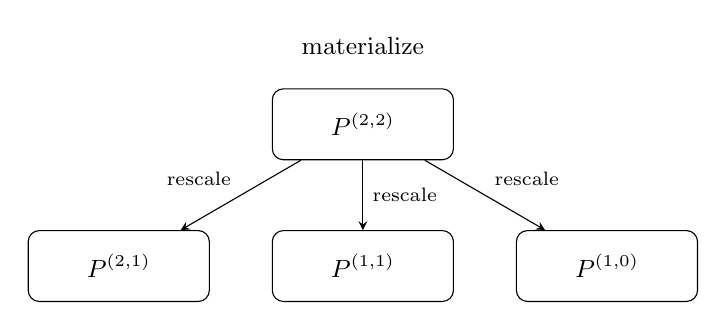
\begin{tikzpicture}[>=stealth, font=\small]
        \node[draw, rounded corners, minimum width=2.3cm, minimum height=0.9cm] (p22) at (0,0) {$P^{(2,2)}$};
        \node[draw, rounded corners, minimum width=2.3cm, minimum height=0.9cm] (p21) at (-3.1,-1.8) {$P^{(2,1)}$};
        \node[draw, rounded corners, minimum width=2.3cm, minimum height=0.9cm] (p11) at (0,-1.8) {$P^{(1,1)}$};
        \node[draw, rounded corners, minimum width=2.3cm, minimum height=0.9cm] (p10) at (3.1,-1.8) {$P^{(1,0)}$};
        \node at (0,1.0) {\small materialize};
        \draw[->] (p22) -- (p21) node[midway, above left] {\scriptsize rescale};
        \draw[->] (p22) -- (p11) node[midway, right] {\scriptsize rescale};
        \draw[->] (p22) -- (p10) node[midway, above right] {\scriptsize rescale};
    \end{tikzpicture}
    \caption{The $R=2$ staircase. Only the base plan $P^{(2,2)}$ is materialized; the remaining three plans are reconstructed from dual differences by row and column rescaling.}
    \label{fig:staircase}
\end{figure}

This reconstruction identity is the signature implementation observation in the manuscript. It converts the explicit four-plan $R=2$ backward into a one-plan materialization plus cheap row and column modifiers, which is why the method maps cleanly to TPU kernels.

\paragraph{Why \texorpdfstring{$R=2$}{R=2}.}
The multiplicative reconstruction itself is not unique to $R=2$. Relative to any chosen base staircase plan, every other staircase plan factors by the corresponding dual differences in the same way. What is special about $R=2$ is that the exact backward closes into the compact four-plan staircase above, so the reconstruction identity yields a practically useful one-base-plan kernel rather than a larger family of rescaled plans.

\subsection{Gap-Aware Dustbin Bridge}

The current gap-aware production path does not use a new OT solver. Instead, it augments the balanced problem. Let the base sequence length be $L$ and let $B=128$ denote the dustbin block size used in the implementation. Define augmented tensors
\[
\widetilde Q,\widetilde K,\widetilde V \in \mathbb{R}^{(L+B)\times d}
\]
by appending one learned dustbin token per side together with $B-1$ inactive filler tokens. The masks are augmented analogously: one appended token is active, the rest are inactive fillers. The implementation then applies the same balanced tail-refinement solver to this augmented system, with effective band width
\[
\widetilde W = \max(W,L).
\]

\begin{proposition}[Dustbin Augmentation Bridge]\label{thm:dustbin_aug}
Let $(\widetilde Q,\widetilde K,\widetilde V,\widetilde\Omega)$ denote the dustbin-augmented tensors and active support constructed above. Then the current \texttt{dustbin\_block} path is exactly the same balanced fixed-support tail-refinement surrogate as in Section~2.2, but applied on the augmented state space.
\end{proposition}

\begin{corollary}[Exact \texorpdfstring{$R=2$}{R=2} Adjoint on the Augmented State Space]\label{cor:dustbin_r2}
Apply Proposition~\ref{prop:tail_adjoint_main} and Theorem~\ref{thm:single_base_main} to the augmented system. Then the current dustbin-augmented transport path inherits the exact fixed-depth adjoint and the same single-base-plan reconstruction on the augmented support.
\end{corollary}

This is the first gap-aware extension carried into the unified paper because it already matches the cloud path. It is a bridge theorem, not a departure from the central balanced factorization.

\subsection{A Local Surrogate-Bias Bound}

The fixed-depth backward is exact for the surrogate it differentiates. A separate question is how far that surrogate gradient can be from the gradient through the full stopped-base computation. Let
\[
z=(u,v),\qquad \Phi_x(z)=z^+,
\]
be the centered one-step refinement map at differentiable parameters $x$, and let $A_x(z)$ denote the transport application map. Write
\[
z_T(x)=\Phi_x^T(z_0),
\qquad
\Psi_x^R(z)=A_x\!\bigl(\Phi_x^R(z)\bigr).
\]
Then the full fixed-depth gradient is
\[
g_{\mathrm{full}}^{T,R}(x)=\nabla_x \Psi_x^R(z_T(x)),
\]
while the stop-gradient surrogate uses
\[
g_{\mathrm{surr}}^{T,R}(x)=\partial_x \Psi_x^R(z)\big|_{z=z_T(x)}.
\]

\begin{theorem}[Local Surrogate-Bias Bound]\label{thm:surrogate_bias}
Assume fixed support, $C^1$ dependence of $\Phi_x$ and $A_x$ on $(x,z)$, and constants $\rho\in[0,1)$, $L_\Phi>0$, and $L_A>0$ such that
\[
\|D_z\Phi_x(z)\|\le\rho,
\qquad
\|D_x\Phi_x(z)\|\le L_\Phi,
\qquad
\|D_z A_x(z)\|\le L_A
\]
on a forward-invariant neighborhood. Then
\[
g_{\mathrm{full}}^{T,R}(x)-g_{\mathrm{surr}}^{T,R}(x)
=
D_z\Psi_x^R(z_T(x))\,D_x z_T(x),
\]
and
\[
\bigl\|g_{\mathrm{full}}^{T,R}(x)-g_{\mathrm{surr}}^{T,R}(x)\bigr\|
\le
\frac{L_A L_\Phi}{1-\rho}\,\rho^R.
\]
\end{theorem}

The point of this bound is modest but useful: once the support is fixed and the refinement map is locally contractive, the stop-gradient bias decays geometrically in the tail depth $R$. Appendix~\ref{app:bias} gives the short proof.

\section{Validation and Experiments}

\subsection{Exactness Validation of the Masked Surrogate}

We first separate surrogate correctness from systems scale. On synthetic masked problems for which exact autodiff through the same centered surrogate remains tractable, we compare the optimized $R=2$ kernel against a pure-JAX reference. Table~\ref{tab:exactness_unified} reports representative maximum absolute gradient deviations under the default validation setting ($\varepsilon=1$, band width $256$, $R=2$).

\begin{table}[h]
    \centering
    \begin{tabular}{@{}rrrr@{}}
        \toprule
        Length $L$ & $\max |\Delta Q|$ & $\max |\Delta K|$ & $\max |\Delta V|$ \\
        \midrule
        $512$ & $1.05 \times 10^{-5}$ & $1.73 \times 10^{-6}$ & $1.06 \times 10^{-9}$ \\
        $1024$ & $5.70 \times 10^{-6}$ & $8.13 \times 10^{-7}$ & $2.55 \times 10^{-10}$ \\
        $2048$ & $5.50 \times 10^{-6}$ & $9.17 \times 10^{-7}$ & $2.29 \times 10^{-10}$ \\
        \bottomrule
    \end{tabular}
    \caption{Maximum absolute gradient deviations between the optimized masked $R=2$ kernel and exact autodiff through the same centered surrogate.}
    \label{tab:exactness_unified}
\end{table}

Additional forward-consistency checks run through lengths $512$, $1024$, $2048$, $4096$, $8192$, and $16384$, with extended spot checks at $32768$, $65536$, and $131072$. We treat the larger checks as forward-consistency evidence rather than as exact-gradient checks.

To calibrate the local surrogate-bias discussion, we also compared tail-refinement gradients against full BPTT through the stopped-base solve on the same synthetic masked setup at $L=512$, $d=8$, $T=15$, $W=256$, and $\varepsilon=1$. Over seeds $0,1,2$, the worst-case gradient discrepancy $\max\{|\Delta Q|,|\Delta K|,|\Delta V|\}$ was $1.49\times 10^{-4}$ for $R=0$, $1.63\times 10^{-5}$ for $R=1$, $1.42\times 10^{-5}$ for $R=2$, and $1.42\times 10^{-5}$ for $R=4$. In this local exact-gradient calibration, the main empirical drop therefore occurs between zero tail refinement and the first one or two refinement steps, while $R=2$ and $R=4$ are already effectively tied at the scale of the masked validation harness.

\subsection{Short Pfam Screen on TPU v6e-8}

The first empirical bridge is the short Pfam screen on TPU v6e-8. All four core configurations complete end-to-end:
\[
\texttt{k2\_eps1},\quad
\texttt{k4\_eps1},\quad
\texttt{muot\_dustbin\_mono},\quad
\texttt{muot\_dustbin\_hybrid}.
\]
Each uses $50{,}000$ training pairs, $T=15$ base iterations, band width $1024$, and global batch size $64$. Table~\ref{tab:screen_unified} reports the step-50 screen snapshot.

\begin{table}[h]
    \centering
    \begin{tabular}{@{}lcccc@{}}
        \toprule
        Config & Step 50 Loss & Step 50 CE & Step 50 Mono & Throughput (ex/s) \\
        \midrule
        \texttt{k2\_eps1} & 3.5778 & 5.3223 & 0.3353 & 8.46 \\
        \texttt{k4\_eps1} & 3.5779 & 5.3223 & 0.3353 & 8.38 \\
        \texttt{muot\_dustbin\_mono} & 3.9030 & 5.3258 & 0.4155 & 8.41 \\
        \texttt{muot\_dustbin\_hybrid} & 4.6250 & 5.3244 & 0.4162 & 8.45 \\
        \bottomrule
    \end{tabular}
    \caption{Short TPU v6e-8 Pfam screen across the four core balanced and dustbin-augmented configurations.}
    \label{tab:screen_unified}
\end{table}

Two immediate conclusions follow. First, on the balanced path we observe no meaningful difference between $R=2$ and $R=4$ at this short-screen budget, while $R=2$ remains slightly faster. Second, the theorem-aligned dustbin bridge is operational at the same systems scale as the balanced path.

\subsection{Promoted Balanced Run}

We then promoted the balanced $\texttt{k2\_eps1}$ configuration to the longer-budget TPU training path. The full objective details are given in the protocol notes in the appendix; for the interpretation of the main text, the important point is that this promotion is a trainability and systems-stability test of the theorem-backed balanced $R=2$ path. The run reached step $1437$, repeatedly synchronized checkpoints to GCS at steps $250$, $500$, $750$, $1000$, and $1250$, and sustained approximately $8.5$ examples per second after startup warmup. The initial throughput at step $0$ was $2.67$ examples per second, after which the run stabilized near $8.5$ examples per second for the remainder of the budget.

This promoted run should therefore be interpreted narrowly but positively. It is strong evidence that the theorem-backed balanced $R=2$ path is stable, efficient, and checkpointable under a realistic TPU budget. The minibatch training loss is not monotone step-by-step, so late fluctuations in scalar loss should be read as ordinary stochastic optimization behavior rather than as an instability signal. The role of this experiment is not to serve as a final downstream alignment benchmark; it is to show that the production theorem-backed path runs cleanly over a long TPU budget.

\section{Discussion}

The unified picture is now clear. The core contribution remains the balanced fixed-support tail-refinement surrogate together with the exact $R=2$ single-base-plan factorization. The dustbin bridge matters because it keeps the first gap-aware extension inside the same theorem family and already matches the current cloud path. The empirical evidence aligns with that theory stack: exactness holds on small masked problems, the four core balanced and dustbin-augmented screen configurations complete on TPU, and the promoted balanced path trains cleanly through a long budget.

What remains outside the present theorem spine should stay outside it. In particular, a genuinely KL-unbalanced transport theorem, differentiable support geometry, and multimodal routing all remain reasonable follow-ons, but they are not required for the central claim of this manuscript.

\paragraph{Limitations and scope.}
The strongest limitations are deliberate. The main theorem is balanced and fixed-support; the dustbin bridge is an augmented balanced construction, not a full KL-unbalanced OT theorem. The local surrogate-bias result is local and contraction-based rather than global. Empirically, the promoted long-budget run is best read as evidence of trainability and systems stability rather than as a final downstream comparison against alternative attention mechanisms or CE-optimized alignment objectives.

\paragraph{Broader context.}
This work is a methods and systems contribution for long-context differentiable alignment. Its immediate positive impact is to make theorem-backed OT attention practical on accelerator hardware. Its main practical costs are computational: the method still requires substantial accelerator time, and the empirical conclusions should be interpreted only within the stated benchmark scope rather than as deployment claims about downstream decision-making systems.

\section{Conclusion}

We presented a single-base-plan backward theory for long-context Sinkhorn attention and carried it through the first gap-aware extension that already matches the production code path. The balanced fixed-support $R=2$ factorization remains the centerpiece. The dustbin augmentation theorem lifts that factorization onto the current gap-aware transport path without changing the underlying surrogate. Exactness validation, a completed four-way TPU screen, and a promoted long-budget balanced run together show that the theorem is not merely algebraic: it maps to a practical TPU training path.

\bibliographystyle{plainnat}
\bibliography{references}

\newpage
\appendix

\section{Balanced Tail-Refinement Proofs}
\label{app:proofs}

\paragraph{Notation.}
For the appendix proofs we work with ungauged representatives satisfying the raw masked logsumexp half-step equations. Let $\Omega$ denote the active support and define
\[
P^{(a,b)}_{ij} =
\begin{cases}
\exp(S_{ij}+u_i^{(a)}+v_j^{(b)}), & (i,j)\in\Omega, \\
0, & (i,j)\notin\Omega.
\end{cases}
\]

\begin{align}
    u_i^{(t+1)} &= -\log\!\Bigl[\sum_{j:(i,j)\in\Omega} \exp(S_{ij} + v_j^{(t)})\Bigr], \label{eq:u_update_app_unified}\\
    v_j^{(t+1)} &= -\log\!\Bigl[\sum_{i:(i,j)\in\Omega} \exp(S_{ij} + u_i^{(t+1)})\Bigr]. \label{eq:v_update_app_unified}
\end{align}

\paragraph{Centering map.}
Let $\mathbf{1}_q$ and $\mathbf{1}_k$ denote the all-ones vectors on valid queries and keys, and let
\[
m = \frac{\mathbf{1}_q}{\mathbf{1}_q^\top\mathbf{1}_q}.
\]
The implementation stores centered representatives via
\[
\mathcal{C}(u,v)=\bigl(u-(m^\top u)\mathbf{1}_q,\; v+(m^\top u)\mathbf{1}_k\bigr).
\]

\begin{lemma}[Centering Pullback]
If $(\bar u,\bar v)$ are cotangents on the outputs of $\mathcal{C}$, then
\[
\mathcal{C}^*(\bar u,\bar v)
=
\Bigl(
\bar u + m\bigl(\mathbf{1}_k^\top \bar v - \mathbf{1}_q^\top \bar u\bigr),
\;
\bar v
\Bigr).
\]
\end{lemma}

\begin{proof}
Write $s=m^\top u$, so $\delta s = m^\top \delta u$. Then
\[
\delta \mathcal{C}(u,v)
=
\bigl(\delta u-(\delta s)\mathbf{1}_q,\; \delta v+(\delta s)\mathbf{1}_k\bigr).
\]
Pairing this variation with $(\bar u,\bar v)$ and collecting coefficients of $\delta u$ and $\delta v$ yields the stated pullback.
\end{proof}

\begin{lemma}[Gauge Equivariance]
Let $\Gamma_c(u,v)=(u-c\mathbf{1}_q,\; v+c\mathbf{1}_k)$. Then the raw two-half-step map defined by equations~\eqref{eq:u_update_app_unified}--\eqref{eq:v_update_app_unified} is gauge equivariant.
\end{lemma}

\begin{proof}
Adding $c$ to every valid key potential shifts every logsumexp argument in the $u$-update by the same constant, so the update subtracts $c$ from every valid query potential. The $v$-update is identical with rows and columns swapped.
\end{proof}

\begin{proposition}[Centered-Ungauged Forward Equivalence]
Let $(\widehat u^{(t)},\widehat v^{(t)})$ be the ungauged iterates and $(u^{(t)},v^{(t)})$ the iterates produced by the centered implementation, both started from the same centered base pair. Then for every $t\ge 1$ there exists a scalar $c_t$ such that
\[
(u^{(t)},v^{(t)})=\Gamma_{c_t}\bigl(\widehat u^{(t)},\widehat v^{(t)}\bigr).
\]
Consequently the centered and ungauged implementations produce exactly the same staircase transport plans.
\end{proposition}

\begin{proof}
The claim holds at $t=1$ by definition of the centering step. Inductively, if the two previous representatives differ by a gauge transform, then gauge equivariance of the raw refinement step shows that the next raw outputs also differ by a gauge transform; applying $\mathcal{C}$ merely chooses another representative of the same orbit.
\end{proof}

\begin{lemma}[Half-Step Jacobians]
For every refinement step $t\ge 1$,
\begin{align}
    \frac{\partial u_i^{(t)}}{\partial v_j^{(t-1)}} &= -P_{ij}^{(t,t-1)}, \\
    \frac{\partial v_j^{(t)}}{\partial u_i^{(t)}} &= -P_{ij}^{(t,t)}.
\end{align}
\end{lemma}

\begin{proof}
Differentiate the masked logsumexp updates. For example,
\[
\frac{\partial u_i^{(t)}}{\partial v_j^{(t-1)}}
=
-
\frac{\exp(S_{ij}+v_j^{(t-1)})}{\sum_{k:(i,k)\in\Omega}\exp(S_{ik}+v_k^{(t-1)})}
=
-\exp(S_{ij}+u_i^{(t)}+v_j^{(t-1)})
=
-P_{ij}^{(t,t-1)}.
\]
The second identity is identical with rows and columns swapped.
\end{proof}

\paragraph{Proof of Proposition~\ref{prop:tail_adjoint_main}.}
\begin{proof}
The direct terminal transport application contributes $P^{(R,R)}\odot Z$ to $\bar S$ together with
\[
\bar v^{(R)}=g_v,
\qquad
\bar u^{(R)}=g_u-P^{(R,R)}\bar v^{(R)}.
\]
Now fix a reverse step $t\in\{1,\dots,R\}$. Pulling $\bar u^{(t)}$ back through the $u$-half-step uses the Jacobian $-P^{(t,t-1)}$:
\[
\bar v^{(t-1)} = -\bigl(P^{(t,t-1)}\bigr)^\top \bar u^{(t)},
\qquad
\bar S \mathrel{-}= P^{(t,t-1)}\odot\bigl(\bar u^{(t)}\mathbf{1}^\top\bigr).
\]
For $t\ge 2$, pulling $\bar v^{(t-1)}$ back through the $v$-half-step uses the Jacobian $-P^{(t-1,t-1)}$:
\[
\bar u^{(t-1)} = -P^{(t-1,t-1)}\bar v^{(t-1)},
\qquad
\bar S \mathrel{-}= P^{(t-1,t-1)}\odot\bigl(\mathbf{1}\bar v^{(t-1)\top}\bigr).
\]
The recursion stops at $\bar u^{(1)}$ because $u^{(0)}$ belongs to the stopped base solve. Summing the direct terminal term with the reverse-time half-step contributions yields equation~\eqref{eq:generic_score_vjp_unified}.
\end{proof}

\paragraph{Proof of Proposition~\ref{thm:single_base_main}.}
\begin{proof}
For any two staircase plans,
\[
\frac{P_{ij}^{(a,b)}}{P_{ij}^{(2,2)}}
=
\exp(u_i^{(a)}-u_i^{(2)}+v_j^{(b)}-v_j^{(2)}),
\]
which gives the exact reconstruction formula immediately. Substituting these reconstructed plans into the explicit $R=2$ score-space VJP leaves every entry unchanged, so the same backward pass can be evaluated while materializing only $P^{(2,2)}$.
\end{proof}

\section{Proofs for the Dustbin Bridge and Surrogate Bias}
\label{app:bias}

\paragraph{Proof of Proposition~\ref{thm:dustbin_aug}.}
\begin{proof}
After constructing the augmented tensors and masks, the implementation calls the same balanced Sinkhorn forward and backward path as in Section~2.2. Because only the first appended token in each dustbin block is active, every transport entry touching the remaining fillers is identically zero. Because the effective band width is $\widetilde W=\max(W,L)$, every active base token can reach the active dustbin token on the opposite side. Thus the implemented path is exactly the balanced fixed-support surrogate on an enlarged state space.
\end{proof}

\paragraph{Proof of Corollary~\ref{cor:dustbin_r2}.}
\begin{proof}
Apply Proposition~\ref{prop:tail_adjoint_main} and Theorem~\ref{thm:single_base_main} to the augmented tensors and support from Theorem~\ref{thm:dustbin_aug}. No new algebra is introduced after the augmentation itself.
\end{proof}

\paragraph{Proof of Theorem~\ref{thm:surrogate_bias}.}
\begin{proof}
By the chain rule,
\[
\nabla_x\Psi_x^R(z_T(x))
=
\partial_x \Psi_x^R(z)\big|_{z=z_T(x)}
+
D_z\Psi_x^R(z_T(x))\,D_x z_T(x),
\]
which gives the exact bias identity after subtracting the partial derivative term.

Next,
\[
D_z\Psi_x^R(z_T(x))
=
D_z A_x(z_{T+R}(x))
\prod_{r=0}^{R-1} D_z\Phi_x(z_{T+r}(x)),
\]
so
\[
\|D_z\Psi_x^R(z_T(x))\|
\le
L_A \rho^R.
\]
Differentiate the base recursion $z_{t+1}(x)=\Phi_x(z_t(x))$:
\[
D_x z_{t+1}(x)
=
D_x\Phi_x(z_t(x))
+
D_z\Phi_x(z_t(x))\,D_x z_t(x).
\]
Because $z_0$ is independent of $x$, repeated application of the norm bounds yields
\[
\|D_x z_T(x)\|
\le
L_\Phi \sum_{j=0}^{T-1}\rho^j
\le
\frac{L_\Phi}{1-\rho}.
\]
Combining the two estimates with the exact bias identity gives
\[
\bigl\|g_{\mathrm{full}}^{T,R}(x)-g_{\mathrm{surr}}^{T,R}(x)\bigr\|
\le
\frac{L_A L_\Phi}{1-\rho}\,\rho^R.
\qedhere
\]
\end{proof}

\section{Experimental Protocol Notes}

The current manuscript uses three empirical layers:
\begin{enumerate}
    \item exactness checks against exact autodiff on small masked problems;
    \item a four-configuration TPU v6e-8 Pfam screen across balanced and dustbin-augmented paths;
    \item a promoted long-budget balanced run for the theorem-backed $R=2$ path.
\end{enumerate}

All TPU results use a single Cloud TPU v6e-8 host. The short screen uses $50{,}000$ Pfam training pairs with the production benchmark stack, and the promoted run uses the same benchmark family at longer budget. The biological inputs and language-model-derived embeddings are pre-existing assets rather than new data collection.

For the promoted balanced run, the objective weights were
\[
\lambda_{\mathrm{rec}}=1,\qquad \lambda_{\mathrm{ce}}=0,\qquad \lambda_{\mathrm{mono}}=0,
\]
so reconstruction loss was optimized directly while CE and monotonicity were logged diagnostically.

An anonymized supplementary code bundle accompanies the submission and contains a single-file kernel implementation for the balanced and dustbin-augmented transport path exercised by the paper. The protocol notes in this appendix record the corresponding run parameters used for the reported TPU configurations.

The main external assets used in the experiments are public Pfam family data and public ESM-2 embeddings. Pfam is distributed under CC0 through the Pfam/InterPro documentation, and the \texttt{esm2\_t6\_8M\_UR50D} weights used for the embeddings are distributed under the MIT license.

The present cloud-aligned gap-aware path is the dustbin-augmented balanced surrogate. Genuinely KL-unbalanced transport and differentiable support geometry remain natural follow-on directions, but they are not needed for the main claim carried by this manuscript.

\section{Kernel-Oriented Pseudocode}

\paragraph{Balanced stopped-base and $R=2$ tail.}
\begin{enumerate}
    \item Form masked scaled scores $S_{ij}=Q_iK_j^\top/(\sqrt{d}\,\varepsilon)$ on the active support $\Omega$.
    \item Run the balanced masked Sinkhorn half-steps for $T$ stopped iterations to obtain the base pair $(u^{(0)},v^{(0)})$.
    \item Recompute two differentiable refinement steps from the stopped base pair, producing $(u^{(1)},v^{(1)})$ and $(u^{(2)},v^{(2)})$.
    \item Materialize only the base staircase plan $P^{(2,2)}$ blockwise.
    \item Reconstruct $P^{(2,1)}$, $P^{(1,1)}$, and $P^{(1,0)}$ by row and column rescaling of $P^{(2,2)}$ using the dual differences $(u^{(a)}-u^{(2)}, v^{(b)}-v^{(2)})$.
    \item Evaluate the exact $R=2$ score-space VJP from Proposition~\ref{prop:tail_adjoint_main} and Theorem~\ref{thm:single_base_main}, then propagate to $(Q,K,V)$.
\end{enumerate}

\paragraph{Dustbin-augmented bridge.}
\begin{enumerate}
    \item Append one active dustbin token per side together with inactive fillers to construct the augmented tensors $(\widetilde Q,\widetilde K,\widetilde V)$.
    \item Augment the masks analogously and enlarge the effective band width to $\widetilde W=\max(W,L)$.
    \item Apply the same balanced stopped-base and $R=2$ tail procedure on the augmented state space.
\end{enumerate}

\section*{NeurIPS Paper Checklist}

\begin{enumerate}

\item {\bf Claims}
    \item[] Question: Do the main claims made in the abstract and introduction accurately reflect the paper's contributions and scope?
    \item[] Answer: \answerYes{}
    \item[] Justification: The abstract and introduction match the proved balanced $R=2$ theorem, the dustbin bridge, the local surrogate-bias bound, the exactness checks, and the reported TPU runs; they do not claim a full KL-unbalanced theory or CE-optimized promoted training.

\item {\bf Limitations}
    \item[] Question: Does the paper discuss the limitations of the work performed by the authors?
    \item[] Answer: \answerYes{}
    \item[] Justification: The discussion explicitly limits the theorem to fixed-support balanced transport, states that the dustbin bridge is not a full unbalanced OT theorem, and notes that the promoted run optimizes reconstruction while CE is diagnostic only.

\item {\bf Theory assumptions and proofs}
    \item[] Question: For each theoretical result, does the paper provide the full set of assumptions and a complete (and correct) proof?
    \item[] Answer: \answerYes{}
    \item[] Justification: The assumptions and statements for the balanced $R=2$ adjoint, the one-reference-tile backward schedule, the dustbin augmentation bridge, the local surrogate-bias bound, the projective contraction certificate, the a posteriori bias certificate, the certified tail-depth optimization rule, and the transport-orbit calculus are given in Section 2, with complete proofs in the appendices.

\item {\bf Experimental result reproducibility}
    \item[] Question: Does the paper fully disclose all the information needed to reproduce the main experimental results of the paper to the extent that it affects the main claims and/or conclusions of the paper (regardless of whether the code and data are provided or not)?
    \item[] Answer: \answerYes{}
    \item[] Justification: The manuscript discloses the exact surrogate, kernel schedule, validation settings, TPU type, dataset family, screen configurations, promoted-run objective weights, throughput, checkpoint steps, and held-out evaluation protocol. The anonymized supplementary ZIP contains the analyzed transport kernel and a Sinkhorn-only Pfam training harness with the reported v6e-8/default settings; it omits cloud launchers, project-specific storage paths, checkpoints, logs, and external data or embedding generation.

\item {\bf Open access to data and code}
    \item[] Question: Does the paper provide open access to the data and code, with sufficient instructions to faithfully reproduce the main experimental results, as described in supplemental material?
    \item[] Answer: \answerYes{}
    \item[] Justification: An anonymized supplementary bundle accompanies the submission and contains the single-file kernel implementation for the balanced and dustbin-augmented transport path plus a Sinkhorn-only Pfam training harness with the reported default settings. It is intended to reproduce and inspect the core kernel/training artifact without cloud launchers or private storage paths. The appendix protocol notes specify the reported run parameters, TPU type, objective settings, and external assets used for the experiments.

\item {\bf Experimental setting/details}
    \item[] Question: Does the paper specify all the training and test details needed to understand the results?
    \item[] Answer: \answerYes{}
    \item[] Justification: The validation section and experimental protocol notes specify the masked validation settings, the four-config TPU screen setup, the promoted-run objective weights, the TPU type, and the main throughput and checkpoint milestones. The supplementary kernel and Sinkhorn-only training harness match the transport path analyzed in the paper.

\item {\bf Experiment statistical significance}
    \item[] Question: Does the paper report error bars suitably and correctly defined or other appropriate information about the statistical significance of the experiments?
    \item[] Answer: \answerNo{}
    \item[] Justification: The empirical evidence is a methods-focused exactness suite, a three-seed local bias-certificate check, an orbit-factorization check, a short TPU screen, and a single promoted run. We do not report multi-seed confidence intervals or other formal significance summaries for the TPU runs.

\item {\bf Experiments compute resources}
    \item[] Question: For each experiment, does the paper provide sufficient information on the computer resources (type of compute workers, memory, time of execution) needed to reproduce the experiments?
    \item[] Answer: \answerYes{}
    \item[] Justification: The paper identifies the TPU v6e-8 platform, reports the short-screen and promoted-run budgets, gives throughput measurements, and states the masked validation scales used for exactness checks.

\item {\bf Code of ethics}
    \item[] Question: Does the research conducted in the paper conform, in every respect, with the NeurIPS Code of Ethics?
    \item[] Answer: \answerYes{}
    \item[] Justification: The work is a methods and systems paper on differentiable attention kernels and benchmark training. It does not involve crowdsourcing, human subjects, or prohibited applications, and the manuscript does not make deployment claims beyond the reported experimental scope.

\item {\bf Broader impacts}
    \item[] Question: Does the paper discuss both potential positive societal impacts and negative societal impacts of the work performed?
    \item[] Answer: \answerYes{}
    \item[] Justification: The discussion limits the claims to factorization-backed trainability and notes the main practical considerations: compute cost, scope of the surrogate, and the difference between reconstruction-optimized and alignment-diagnostic quantities.

\item {\bf Safeguards}
    \item[] Question: Does the paper describe safeguards that have been put in place for responsible release of data or models that have a high risk for misuse (e.g., pretrained language models, image generators, or scraped datasets)?
    \item[] Answer: \answerNA{}
    \item[] Justification: The submission does not release a high-risk generative model or a new scraped dataset; it studies transport-based attention kernels and benchmark training methodology.

\item {\bf Licenses for existing assets}
    \item[] Question: Are the creators or original owners of assets used in the paper properly credited and are the license and terms of use explicitly mentioned and properly respected?
    \item[] Answer: \answerYes{}
    \item[] Justification: The protocol notes identify the public Pfam data and the public ESM-2 weights used in the experiments and state the license information included in the submission text: CC0 for Pfam/InterPro and MIT for the ESM-2 checkpoint used for embeddings.

\item {\bf New assets}
    \item[] Question: Are new assets introduced in the paper well documented and is the documentation provided alongside the assets?
    \item[] Answer: \answerNA{}
    \item[] Justification: The submission does not introduce a new public dataset or model asset release.

\item {\bf Crowdsourcing and research with human subjects}
    \item[] Question: For crowdsourcing experiments and research with human subjects, does the paper include the full text of instructions given to participants and screenshots, if applicable, as well as details about compensation (if any)?
    \item[] Answer: \answerNA{}
    \item[] Justification: The paper does not involve crowdsourcing or human-subject experiments.

\item {\bf Institutional review board (IRB) approvals or equivalent for research with human subjects}
    \item[] Question: Does the paper describe potential risks incurred by study participants, whether such risks were disclosed to the subjects, and whether Institutional Review Board (IRB) approvals (or an equivalent approval/review based on the requirements of your country or institution) were obtained?
    \item[] Answer: \answerNA{}
    \item[] Justification: The paper does not involve human-subject research.

\item {\bf Declaration of LLM usage}
    \item[] Question: Does the paper describe the usage of LLMs if it is an important, original, or non-standard component of the core methods in this research? Note that if the LLM is used only for writing, editing, or formatting purposes and does \emph{not} impact the core methodology, scientific rigor, or originality of the research, declaration is not required.
    \item[] Answer: \answerNA{}
    \item[] Justification: LLMs are not part of the core method, proofs, experimental protocol, or scientific claims in this submission.

\end{enumerate}


\end{document}
